% assignment_4.tex
% CS 8735 - Unsupervised Learning (Fall 2015)
%     University of Missouri-Columbia
%             Chanmann Lim
%            November 2015

\documentclass[a4paper]{article}

\usepackage[margin=1 in]{geometry}
\usepackage{listings}
\usepackage{amsmath}
\usepackage{graphicx}
\usepackage{float}

\everymath{\displaystyle}
\DeclareMathOperator*{\argmax}{\arg\!\max}
\DeclareMathOperator*{\argmin}{\arg\!\min}

\begin{document}
\title{CS 8735: Report for assignment 4}
\author{Chanmann Lim}
\date{November 12, 2015}
\maketitle

\noindent The Matlab code for all experiments is in the \textbf{Appendix} section.

\paragraph{Problem 1.} In this task, we are going carry out spectral clustering on synthetic Circle.dat dataset. The first step in spectral clustering is to construct sparse graph by considering each data-point as a vertex of the Graph G(V,E) then connect two vertices that have the squared Euclidean distance smaller than $\epsilon = 1.5$. Creating an edge $e_{ij}$ when

\begin{equation}
	||x_i-x_j||^2 < \epsilon  \quad     \forall i,j
\end{equation}

Then using this sparse graph to generate n-by-n W matrix where n is the size of the dataset and $w(i, j)$ , the element at row $i^{th}$ and column $j^{th}$ is defined as

\begin{equation}
	w(i, j) = e^{\frac{-||x_i-x_j||^2}{\sigma^2}} \quad \text{if e\textsubscript{ij} exists and 0 otherwise}
\end{equation}

where $\sigma^2=2$, then we compute diagonal D matrix where each diagonal element Dii is the significance of each vertex:

\begin{equation}
	D_{ii}= \sum_{j\in V} w(i,j)
\end{equation}

Next, we define the graph Laplacian matrix $L = D – W$ and perform transformation on L to get normalized graph Laplacian matrix $\tilde{L}=D^{-1/2} LD^{-1/2}$ finally we can carry out eigen analysis on the normalized graph Laplacian matrix to obtain the eigenvalues and eigenvectors for our clustering task.

\paragraph{a)} The smallest five eigenvalues we got are [0, 0.0002, 0.0024, 0.0083, 0.0158].
\paragraph{b)} In minimizing the normalized cut spectral clustering pushes the smallest eigenvalue to zero hence it is no longer be appropriate for clustering task and we have to use the eigenvector $z_1$ that corresponding to the first non-zero eigenvalue to compute $y_1=D^{-1/2} z_1$ then assign $x_i$ to cluster C1 if $y_i < median (y)$ otherwise assign $x_i$ to cluster C2.

  \begin{figure}[H]
    \centering
      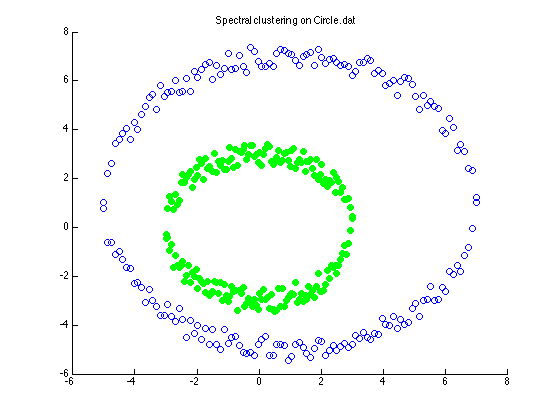
\includegraphics[scale=.47]{images/1.png}
    \caption{Plot of cluster assignment}
  \end{figure}

\paragraph{Problem 2.} In language modeling training, given four commands and a list of eight words we are going carry out latent semantic analysis by employing singular value decomposition (SVD) to transform the W (word by document) matrix into a smooth representation or concept of document namely "scaled document vectors" then we are going to merge a new test document and project its scaled document vector by mean of "fold-in" method and finally to compute the Euclidean distance between the new test command and the existing commands then rank them accordingly.

\paragraph{a)} $W_{8\times4}$ matrix is constructed such that its element $W_{ij} = (1-\epsilon_i)\frac{C_{ij}}{n_j}$ where $C_{ij}$ is the numbers of $word_i$ occurred in $document_j$, $n_j$ is the numbers of words in $document_j$ and $\epsilon_i$ is the normalized entropy of $word_i$ in the training set.

\begin{align}
	\epsilon_i &= \frac{-\sum_{j=1}^N \frac{C_{ij}}{t_i} \log \frac{C_{ij}}{t_i}}{-\sum_{j=1}^N \frac{1}{N} \log \frac{1}{N}} \\
		&= -\frac{1}{\log N} \sum_{j=1}^N \frac{C_{ij}}{t_i} \log \frac{C_{ij}}{t_i}
\end{align}

and $t_i = \sum_{j=1}^N C_{ij}$ with log being log base 2 when computing $\epsilon_i$. We obtain:

\begin{equation}
	W = \begin{bmatrix}
            0.0519  &  0.0519  &  0.0415   &      0 \\
		    0.0519  &  0.0519  &  0.0415   &      0 \\
	        0       &  0       &  0        & 0 \\
			0.1250  &       0  &  0.1000   &      0 \\
			0   & 0.2500   &     0         & 0 \\
			0   &      0   & 0.1000  &  0.1667 \\
			0   &      0   &     0   & 0.3333 \\
			0   &      0   &     0   &      0
        \end{bmatrix}
\end{equation}

\paragraph{b)} Next we decompose W by carry out SVD decomposition $W = U_RS_RV_R^T$ and we obtain:

\begin{equation}
	U_R = \begin{bmatrix}
			0.0200 &  -0.2450  &  0.2798 &   0.1085 \\
			0.0200 &  -0.2450  &  0.2798 &   0.1085 \\
			0.0000 &   0.0000  & -0.0000 &   0.0000 \\
			0.0449 &  -0.1263  &  0.8121 &   0.2857 \\
			0.0066 &  -0.9280  & -0.2760 &  -0.0484 \\
			0.4768 &  -0.0313  &  0.2636 &  -0.8380 \\
			0.8774 &   0.0416  & -0.1955 &   0.4362 \\
			0      &   0       &  0      &   0
		\end{bmatrix}
\end{equation}

\begin{equation}
	S_R = \begin{bmatrix}
			 0.3759   &      0    &     0    &     0 \\
		     0  &  0.2633   &      0  &       0 \\
		     0  &       0   & 0.1903  &       0 \\
		     0  &       0   &      0  &  0.0662
		\end{bmatrix}
\end{equation}

\begin{equation}
	V_R = \begin{bmatrix}
			0.0204 &  -0.1565 &   0.6862  &  0.7101 \\
			0.0099 &  -0.9776 &  -0.2100  & -0.0128 \\
			0.1432 &  -0.1371 &   0.6875  & -0.6986 \\
			0.9894 &   0.0329 &  -0.1116  & 0.0866
		\end{bmatrix}
\end{equation}
	
\paragraph{c)} By keeping the eigenvectors corresponding to the largest tow eigenvalues and computing the scaled document vectors of the four documents with $\bar{V}=S_RV_R^T$ we obtain dimension reduction in document smooth representation.

\begin{equation}
	\bar{V_2} = \begin{bmatrix}
			0.0077  &  0.0037  &  0.0538  &  0.3719 \\
			-0.0412 &  -0.2574 &  -0.0361 &   0.0087
		\end{bmatrix}
\end{equation}

\paragraph{d)} For the new test document we use "fold-in" method to compute $\bar{v_2}(5) = U_{8\times 2}^T \tilde{d_5}$ where $\tilde{d_5} = (1-\epsilon_i)\frac{C_{i5}}{n_5}$ and we obtain:

\begin{equation}
	\bar{v_2}(5) = \begin{bmatrix}
			    0.0606 \\
			   -0.0166
		\end{bmatrix}
\end{equation}

\paragraph{e)} Finally we compute the Euclidean distance between the test command (d-5) and the training commands using their scaled document vector.

\begin{center}
    \begin{tabular}{ |c |c |c |c |c | }
      \hline
       & d-1 & d-2 & d-3 & d-4 \\ \hline
      d-5 &     0.0584  &  0.2474  &  0.0206 &   0.3123 \\ \hline
    \end{tabular}
\end{center}

Hence the closest neighbors of d-5 rank from d-3, d-1, d-2 and d-4 sequentially.

  \begin{figure}[H]
    \centering
      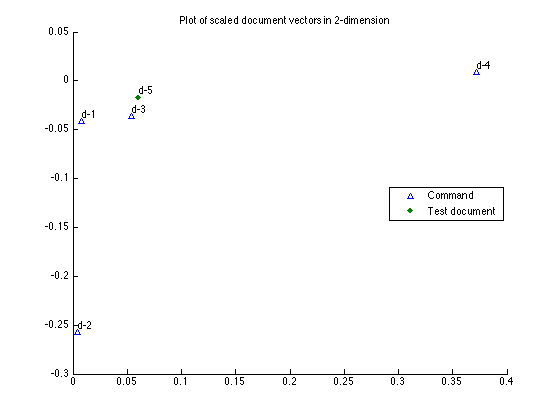
\includegraphics[scale=.57]{images/doc_vecs.png}
    \caption{Plot of scaled document vector in 2-dimension}
  \end{figure}

\paragraph{Problem 3.} Given a Euclidean distance matrix of five data samples, we are going to use classical multidimensional scaling (MDS) algorithm to estimate the 2-D coordinates of the five data-points. In MDS we begin by squaring the elements of the Euclidean distance matrix then perform double centering on the squared distance matrix with $J = \mathbf{I}_n - \frac{1}{n}\mathbf{1}_n\mathbf{1}_n^T$ to obtain $B_\Delta = -\frac{1}{2}JD^{(2)}J$ then we carry out eigen decomposition of $B_\Delta = V\Lambda V^T$. We finally choose the two largest positive eigenvalues and their corresponding eigenvectors to form approximation for the five data samples by computing $\hat{X} = V_{+}\Lambda_{+}^{\frac{1}{2}}$.

\paragraph{a)} The result of eigenvalue matrix $\Lambda_{+}$, eigenvector matrix $V_{+}$ and the estimated coordinates $\hat{X}$ are:

\begin{equation}
	\Lambda_{+} = \begin{bmatrix}
			        4.0000   &      0 \\
         			0  &  2.8000
		\end{bmatrix}
\end{equation}

\begin{equation}
	V_{+} = \begin{bmatrix}
			    0.5000  & -0.4781 \\
			    0.5000  &  0.1195 \\ 
			   -0.0000  &  0.7171 \\
			   -0.5000  &  0.1195 \\
			   -0.5000  & -0.4781
		\end{bmatrix}
\end{equation}

\begin{equation}
	\hat{X} = \begin{bmatrix}
				    1.0000  & -0.8000 \\
				    1.0000  &  0.2000 \\
				   -0.0000  &  1.2000 \\
				   -1.0000  &  0.2000 \\
				   -1.0000  & -0.8000
		\end{bmatrix}
\end{equation}

\paragraph{b)} To verify that the estimated data coordinates are centered we compute the mean of $\hat{X}$ and it in fact yield the values very close to zeros due to numerical computation precision bias. We also recover the Euclidean distance matrix from the projected data samples $\hat{X}$ and confirm the exact match with the original distance matrix.

\begin{equation}
	\hat{D} = \begin{bmatrix}
		        0  &  1.0000  &  2.2361  &  2.2361  &  2.0000 \\
			    1.0000  &       0  &  1.4142  &  2.0000  &  2.2361 \\
			    2.2361  &  1.4142  &       0  &  1.4142  &  2.2361 \\
			    2.2361  &  2.0000  &  1.4142  &       0  &  1.0000 \\
			    2.0000  &  2.2361  &  2.2361  &  1.0000  &       0
		\end{bmatrix}
\end{equation}

\paragraph{Problem 4.} In this experiment, we are going to evaluate the quality of clusters by computing the mutual information(MI) and normalized mutual information(NMI) by the following equations:

\begin{equation}
	MI = \sum_i \sum_j P_{ij} \log_2 \frac{P_{ij}}{P_iP_j}
\end{equation}

\begin{equation}
	NMI = \frac{MI}{\sqrt{H(X)H(Y)}}
\end{equation}

where $P_{ij}$ is the probability of x being assigned to cluster j and it belongs to class i, $P_i$ is the probability of x belongs to class i, and $P_j$ is the probability of x being assigned to cluster j and $H$ is the entropy.

\begin{equation}
	H(X) = -\sum_i P_i \log_2 Pi
\end{equation}

Hence we obtain:

\begin{center}
    \begin{tabular}{ |c |c |c |c | }
      \hline
       & a & b & c \\ \hline
       MI & 0.9799 & 0.4067 & 0.0718 \\ \hline
       NMI & 1 & 0.4562 & 0.0733 \\ \hline
    \end{tabular}
\end{center}

We observed that both MI and NMI provide accurate performance measurement for cluster quality evaluation. In cluster labels (a) case it proves that MI and NMI are indeed insensitive to cluster labeling name and yield the highest values among other cases. The cluster labels (b) has higher MI and NMI then cluster labels (c) since it makes only two clustering mistakes for $x_1$ and $x_2$ comparing four mistakes occurred in (c). This have shown that the higher the values of MI and NMI the better the clustering quality is.

\newpage
\subsection*{Appendix:}
	\lstinputlisting[language=Matlab, title=\lstname, basicstyle=\footnotesize]{assignment_4.m}
	\lstinputlisting[language=Matlab, title=\lstname, basicstyle=\footnotesize]{problem_1.m}
	\lstinputlisting[language=Matlab, title=\lstname, basicstyle=\footnotesize]{problem_2.m}
	\lstinputlisting[language=Matlab, title=\lstname, basicstyle=\footnotesize]{problem_3.m}
	\lstinputlisting[language=Matlab, title=\lstname, basicstyle=\footnotesize]{problem_4.m}
	\lstinputlisting[language=Matlab, title=\lstname, basicstyle=\footnotesize]{problem_1.m}
	\lstinputlisting[language=Matlab, title=\lstname, basicstyle=\footnotesize]{Prob.m}
	\lstinputlisting[language=Matlab, title=\lstname, basicstyle=\footnotesize]{entropy.m}
\end{document}